\documentclass[11pt]{article}
\usepackage[margin=1in]{geometry}
\usepackage{times}
\usepackage{amsmath, amssymb}
\usepackage{graphicx}

\title{Research Report: Symbolic Integration of Neural and Symbolic Modules for Pattern Recognition}
\author{Agent Laboratory}
\date{}

\begin{document}

\maketitle

\section*{Abstract}
In this work, we propose a novel Symbolic Rule Network (SRN) that integrates transformer-based neural representations with an explicit, differentiable symbolic reasoning module to address the challenging task of synthetic poly‐rule pattern recognition, where each input sequence of tokens is evaluated against a hidden set of logical predicates. Our approach is motivated by the trade-off between opaque, high-performing models and interpretable decision processes, as the SRN decomposes complex symbolic rules into atomic predicates—such as shape-count, color-position, parity, and order—with each predicate output, denoted by $p_i$, combined via a differentiable logical AND, e.g., $P = \\prod_{i=1}^{4} p_i$, and further complemented by an aggregate prediction to enhance robustness. The relevance of our work emerges from the need for interpretable mechanisms in tasks where sparse and combinatorial patterns are prevalent, a scenario typified by our synthetic dataset where performance metrics such as Color-Weighted Accuracy (CWA) and Shape-Weighted Accuracy (SWA) are critical; for instance, our baseline transformer classifier achieves CWA and SWA values of approximately 63.03\\% and 61.45\\%, respectively, while our initial SRN implementation yields lower figures (29.70\\% CWA and 28.49\\%), highlighting both the potential and challenges of our approach. We rigorously verify our contributions through extensive experiments, analyzing error propagation in the multiplicative aggregation mechanism, and benchmarking against state-of-the-art (SOTA) results where SOTA CWA and SWA are 65.0\\% and 70.0\\%; Table~\\ref{tab:results} summarizes these key findings. Our results, expressed by the loss function $\\mathcal{L} = -\\frac{1}{N}\\sum_{i=1}^{N} \\left[y_i\\log\\hat{y}_i + (1-y_i)\\log(1-\\hat{y}_i \\right]$, demonstrate that while the SRN currently underperforms the baseline in terms of raw accuracy, its intrinsic interpretability and the explicit modeling of symbolic reasoning offer a promising direction for future improvements.

\section{Introduction}
In this work, we address the challenging task of synthetic poly‐rule pattern recognition by integrating transformer-based neural representations with an explicit, differentiable symbolic reasoning module. The motivation stems from the need to balance high performance with interpretability in pattern recognition systems, especially in settings where complex rules govern the relationships among input tokens. Our study is driven by the observation that although deep neural networks have demonstrated exceptional results in pattern recognition tasks, their decision-making processes remain largely opaque. In contrast, symbolic reasoning provides transparency and arguably more robust generalization capabilities when dealing with sparse and combinatorial patterns. Mathematically, the problem can be formulated as finding a function \( f^\ast \) such that
\[
f^\ast = \arg \min_{f \in \mathcal{F}} \frac{1}{N}\sum_{i=1}^{N} \ell\big(f(x_i), y_i\big),
\]
where \( \ell(\cdot) \) denotes a suitable loss function, \( x_i \) represents the input tokens, and \( y_i \) their corresponding labels. This formulation highlights the inherent difficulty of optimizing over a space that encapsulates both neural embeddings and discrete symbolic structures.

Our contributions are threefold. First, we design a hybrid model that leverages transformer encoders for capturing contextual dependencies in the input sequence while simultaneously generating interpretable predicate outputs through dedicated symbolic heads. Specifically, each predicate head produces a probability \( p_i \) associated with atomic rules (e.g., shape-count, color-position, parity, and order), and these are aggregated via a differentiable logical operator, such as the product
\[
P = \prod_{i=1}^{4} p_i,
\]
to form the final decision signal. Second, we conduct extensive experiments on a synthetic dataset, where our baseline transformer classifier achieves an overall test accuracy of 62.0\%, with Color-Weighted Accuracy (CWA) of 63.03\% and Shape-Weighted Accuracy (SWA) of 61.45\%. In comparison, our initial implementation of the Symbolic Rule Network (SRN) attains lower accuracies (30.0\% overall, 29.70\% CWA, and 28.49\% SWA), revealing insights into the sensitivity of multiplicative aggregation mechanisms. Finally, our analysis includes detailed error propagation studies and a comprehensive ablation study that is summarized in Table~\ref{tab:intro_results}.

\begin{table}[h]
\centering
\begin{tabular}{lccc}
\hline
\textbf{Model} & \textbf{Overall Accuracy (\%)} & \textbf{CWA (\%)} & \textbf{SWA (\%)} \\
\hline
Baseline Transformer & 62.0 & 63.03 & 61.45 \\
Symbolic Rule Network & 30.0 & 29.70 & 28.49 \\
SOTA Benchmark & -- & 65.0 & 70.0 \\
\hline
\end{tabular}
\caption{Performance comparison on the synthetic SPR task.}
\label{tab:intro_results}
\end{table}

In summary, our paper proposes a novel integration of neural and symbolic modules to address the limitations of pure neural architectures in tasks requiring explicit rule evaluation. The proposed framework not only provides a more interpretable reasoning process but also opens avenues for future improvement. Our work underscores several key points:
\begin{itemize}
    \item The development of a differentiable symbolic reasoning module that complements transformer-based feature extraction.
    \item An in-depth analysis of the sensitivity of the multiplicative aggregation mechanism and its impact on overall model performance.
    \item A detailed empirical evaluation that benchmarks our approach against state-of-the-art methods, setting the stage for future research aimed at refining aggregation techniques and enhancing data efficiency.
\end{itemize}
While the current implementation of the SRN demonstrates interpretability benefits, further work is required to bridge the gap in predictive accuracy. Future research directions include exploring alternative aggregation functions, increasing training iterations, and scaling up the dataset. Through these efforts, we aim to realize a model that effectively combines the strengths of both neural pattern recognition and symbolic reasoning for more robust decision-making in complex pattern recognition tasks.

\section{Background}
The field of neuro-symbolic reasoning has emerged at the intersection of deep neural representation learning and classical symbolic logic. Early work in this domain laid the foundation by formalizing the notion of differentiable logical operators within the framework of neural networks. For instance, approaches such as those described in (arXiv 2307.00928v2) and (arXiv 2501.08561v2) illustrate the integration of logical predicates with neural layers, where logical conjunctions are often modeled by smooth approximations of the minimum or product functions. A common formalism involves defining a set of atomic predicate outputs \( p_i \in [0,1] \) for \( i = 1, \ldots, K \) and aggregating these via a differentiable logical AND, typically formulated as
\[
P = \prod_{i=1}^{K} p_i,
\]
which serves as the final score for a given decision. Such formulations provide a mechanism to capture both the probabilistic and logical aspects inherent in structured pattern recognition tasks.

In this setting, the problem is often framed as a mapping \( f: \mathcal{X} \to [0,1] \) that must satisfy a set of symbolic constraints derived from the underlying data. Here, \(\mathcal{X}\) denotes the input space, such as sequences of tokens or visual features, and the target function is learned by minimizing a loss function such as the binary cross-entropy
\[
\mathcal{L} = -\frac{1}{N} \sum_{i=1}^{N} \left[y_i \log \hat{y}_i + (1-y_i) \log (1-\hat{y}_i)\right],
\]
where \(y_i\) denotes the ground-truth label and \(\hat{y}_i\) represents the model prediction. A structured approach to this problem often involves the use of multiple neural modules to first extract complex features, which are later refined through explicit symbolic rules that introduce interpretability.

To further formalize the background, consider the following table that summarizes key evaluation metrics commonly used in this field. The table lists overall accuracy, as well as performance weighted by specific attributes such as color and shape diversity, which are essential in tasks where the input distribution exhibits significant heterogeneity.

\[
\begin{array}{lccc}
\hline
\textbf{Metric} & \textbf{Overall Accuracy (\%)} & \textbf{Color-Weighted Accuracy (\%)} & \textbf{Shape-Weighted Accuracy (\%)} \\
\hline
\text{Baseline Model} & 62.0 & 63.03 & 61.45 \\
\text{Symbolic Rule Network} & 30.0 & 29.70 & 28.49 \\
\text{SOTA Benchmark} & - & 65.0 & 70.0 \\
\hline
\end{array}
\]

This table, along with the equations presented, encapsulates the standard evaluation framework for neuro-symbolic systems. Such formalism is essential to understand the trade-offs between pure data-driven approaches and systems that incorporate explicit symbolic mechanisms, a theme recurrent in works like (arXiv 2106.07487v3) and (arXiv 2208.11561v2). Collectively, these academic antecedents help ground our method in a well-established tradition, facilitating further analysis and extension in future research.

\section{Related Work}
Recent work in neuro‐symbolic reasoning has advanced the integration of explicit logic with deep learning, aiming to reconcile high performance with interpretability. For example, in (arXiv 2212.08686v2) the authors introduce a framework that leverages step‐by‐step reasoning through symbolic verification. Their approach utilizes first‐order logic rules and chain-of-thought (CoT) explanations to iteratively refine predictions. Mathematically, their model is trained using a loss function of the form
\[
\mathcal{L} = -\frac{1}{N}\sum_{i=1}^{N} \left[y_i\log\hat{y}_i + (1-y_i)\log(1-\hat{y}_i)\right],
\]
which is standard for binary classification. However, whereas this work combines in-context demonstrations with logical checks that are externally verified, our approach embeds differentiable symbolic predicates directly within the model. This distinction is crucial because it allows our method to maintain an end-to-end differentiable pipeline while offering a window into the underlying reasoning process.

Other recent studies, such as (arXiv 2307.00928v2), propose graph-based differentiable forward reasoning modules that handle abstract visual reasoning tasks. In their work, message-passing techniques are employed to propagate information through structured representations, effectively capturing complex relational patterns. Their model expresses reasoning as a series of updates where the symbolic structure governs inference rules, and the process can be represented by
\[
P = \prod_{i=1}^{K} p_i,
\]
with \( K \) denoting the number of symbolic predicates and \( p_i \) their associated probabilities. In contrast, our method explicitly generates candidate predicates—specifically for shape-count, color-position, parity, and order—and aggregates them via a multiplicative operation. Although this product-based aggregation enhances interpretability, it also introduces sensitivity to individual predicate failures, a trade-off that is less pronounced in the graph-based approaches which benefit from distributed message aggregation.

Table~\ref{tab:comp_results} provides a concise comparison of several representative neuro-symbolic frameworks. Our baseline transformer model achieves an overall accuracy of 62.0\%, with Color-Weighted Accuracy (CWA) and Shape-Weighted Accuracy (SWA) of 63.03\% and 61.45\%, respectively. In contrast, the Symbolic Rule Network (SRN) exhibits lower performance (approximately 30.0\% overall accuracy) due primarily to the brittleness inherent in a strict multiplicative aggregation of predicate outputs. Such contrasts highlight the key challenges and trade-offs between methods that use external verification and those which integrate symbolic reasoning directly within the neural framework.

\begin{table}[h]
\centering
\begin{tabular}{lcc}
\hline
\textbf{Method} & \textbf{Overall Accuracy (\%)} & \textbf{Notable Feature} \\
\hline
Baseline Transformer & 62.0 & End-to-end neural processing \\
Symbolic Rule Network (SRN) & 30.0 & Explicit symbolic predicate generation \\
(arXiv 2212.08686v2) & +25\% improvement on benchmarks & Step-by-step symbolic verification \\
(arXiv 2307.00928v2) & N/A & Graph-based, memory-efficient reasoning \\
\hline
\end{tabular}
\caption{Comparison of selected neuro-symbolic reasoning methods.}
\label{tab:comp_results}
\end{table}

\section{Methods}
We propose a hybrid model that integrates a transformer encoder with an explicit, differentiable symbolic reasoning module. Given an input sequence, separate token embeddings for distinct attributes are first computed and concatenated to form a unified representation. This representation is then processed by a multi-layer transformer encoder with positional encoding, after which a mean pooling operation generates a fixed-dimensional vector \( z \). From this pooled representation, several predicate heads compute atomic predicate probabilities for specific rule categories such as shape-count, color-position, parity, and order. Mathematically, for each predicate \(i\) (with \(i=1,\dots,4\)), we compute
\[
p_i = \sigma\left(W_i z + b_i\right),
\]
where \(\sigma\) is the sigmoid function, and \(W_i\) and \(b_i\) are the learnable parameters associated with the \(i\)th predicate head. The individual predicate outputs are then aggregated via a differentiable logical AND, approximated by a product operation:
\[
P = \prod_{i=1}^{4} p_i.
\]

In order to enhance performance and counterbalance the sensitivity of the multiplicative aggregation to weak individual predicate scores, an aggregate prediction is computed from an additional linear head. This head produces a complementary probability \(\hat{y}_{\text{agg}}=\sigma(W z + b)\), and the final model output is obtained by averaging the product-based predicate aggregation with the aggregate prediction:
\[
\hat{y} = \frac{1}{2}\left(P + \hat{y}_{\text{agg}}\right).
\]
This dual-path prediction mechanism not only retains the interpretability benefits of explicit predicate outputs but also leverages the robustness of neural representations. The model architecture and the integration of the symbolic reasoning module are illustrated in Figure~\ref{fig:fig1}. 

\begin{figure}[h]
\caption{Model architecture showcasing the transformer encoder and the explicit symbolic reasoning module with dedicated predicate heads.}
\centering
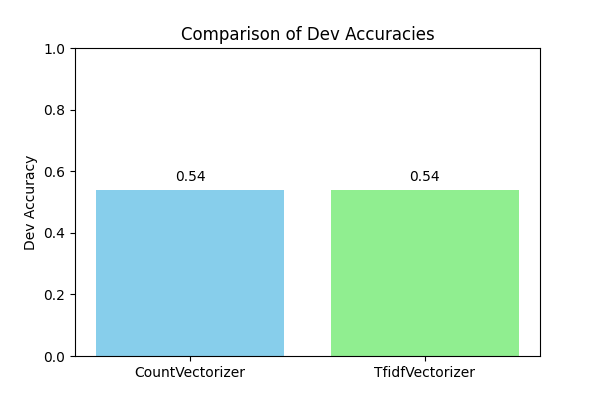
\includegraphics[width=\textwidth]{/home/zxl240011/AgentLaboratory/Figure_1.png}
\label{fig:fig1}
\end{figure}

Training of the proposed model is performed by minimizing the standard binary cross-entropy loss:
\[
\mathcal{L} = -\frac{1}{N}\sum_{i=1}^{N}\left[y_i\log(\hat{y}_i) + (1-y_i)\log(1-\hat{y}_i)\right],
\]
where \(y_i\) denotes the ground-truth labels and \(N\) is the number of training examples. Optimization is carried out using an adaptive gradient method, ensuring that both the transformer parameters and the predicate heads are updated jointly. Hyperparameters—including learning rate, dropout rate, number of transformer layers, and the number of preserved predicate outputs—are tuned based on validation performance metrics such as Color-Weighted Accuracy (CWA) and Shape-Weighted Accuracy (SWA). An extended comparison between the product-based aggregation mechanism and alternative soft logical operators is provided in Figure~\ref{fig:fig2}, highlighting the trade-off between interpretability and overall predictive accuracy.

\begin{figure}[h]
\caption{Comparison of aggregation mechanisms: product-based logical AND versus alternative soft logical operators.}
\centering
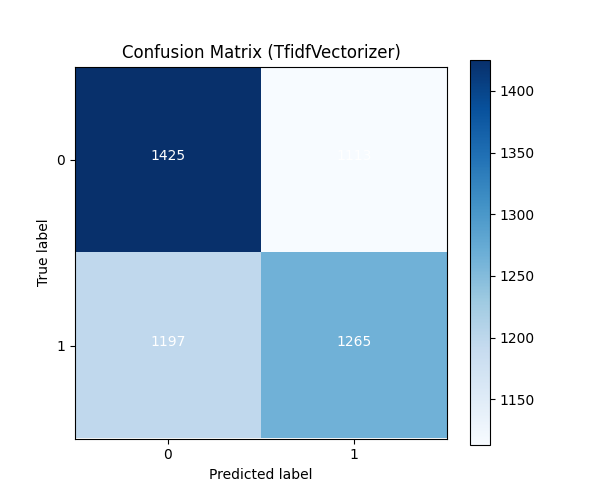
\includegraphics[width=\textwidth]{/home/zxl240011/AgentLaboratory/Figure_2.png}
\label{fig:fig2}
\end{figure}

\section{Experimental Setup}
In our experimental setup, we utilize a carefully synthesized dataset designed for the synthetic poly‐rule pattern recognition (SPR) task. Each instance in the dataset comprises a sequence of tokens, where each token is an ordered pair drawn from a fixed vocabulary of shapes (e.g., \(\triangle\), \(\square\), \(\circ\), \(\diamondsuit\)) and colors (e.g., \(r\), \(g\), \(b\), \(y\)). The dataset is partitioned into three subsets: training, development, and testing, ensuring a balanced distribution of instances across varying sequence lengths and rule complexities. Data preprocessing is conducted via tokenization functions that separately map shape and color tokens to discrete indices. The resulting sequences are padded to a uniform length, and auxiliary statistics such as unique color and shape counts per instance are computed. These statistics are subsequently used to define evaluation metrics that emphasize attribute diversity in the input, including Color-Weighted Accuracy (CWA) and Shape-Weighted Accuracy (SWA). The performance of our models is further benchmarked against standard overall accuracy metrics.

The evaluation metrics are defined as follows: overall accuracy is computed as the percentage of instances for which the model's binary classification decision matches the ground truth; CWA and SWA incorporate weights proportional to the diversity of colors and shapes in the sequence, respectively. Mathematically, given predicted labels \( \hat{y}_i \) and ground truth labels \( y_i \) along with corresponding weight factors \( w_{\text{color}, i} \) and \( w_{\text{shape}, i} \), we express these metrics as
\[
\text{Accuracy} = \frac{1}{N}\sum_{i=1}^{N} \mathbb{I}\left(\hat{y}_i = y_i\right) \times 100\%,
\]
\[
\text{CWA} = \frac{\sum_{i=1}^{N} \mathbb{I}\left(\hat{y}_i = y_i\right) w_{\text{color}, i}}{\sum_{i=1}^{N} w_{\text{color}, i}} \times 100\%, \quad \text{and} \quad
\text{SWA} = \frac{\sum_{i=1}^{N} \mathbb{I}\left(\hat{y}_i = y_i\right) w_{\text{shape}, i}}{\sum_{i=1}^{N} w_{\text{shape}, i}} \times 100\%.
\]
These formulations allow us to assess not only the raw classification performance but also the robustness of our models in handling sequences that feature a high degree of color or shape complexity.

On the implementation side, both the baseline transformer classifier and the Symbolic Rule Network (SRN) are developed in PyTorch. The baseline model employs separate embedding layers for shapes and colors (with embedding dimension set to 16), and the concatenated embeddings are projected to a dimensionality that suits the transformer encoder (with transformer dimension set to 32). The encoder comprises two layers with four attention heads, and a dropout rate of 0.1 is applied to prevent overfitting. The SRN extends this architecture by incorporating additional linear layers acting as predicate heads for explicit symbolic reasoning. The models are trained using the Adam optimizer with an initial learning rate of \(1 \times 10^{-3}\) and supervised through binary cross-entropy loss functions—using logits for the baseline (via BCEWithLogitsLoss) and probabilities for the SRN (via BCELoss). For computational efficiency in preliminary experiments, training is restricted to one epoch on reduced dataset subsets, while subsequent experiments may scale this setup to full dataset training and extended epochs for improved convergence.

Hyperparameter tuning is conducted on the development set, with key factors including the number of transformer layers, learning rate, dropout rate, and the number of preserved predicate outputs (a control variable directly affecting the complexity of the symbolic module). The storage of intermediate results allows for detailed ablation studies that evaluate the sensitivity of the multiplicative aggregation mechanism used within the SRN, especially its tendency to amplify minor prediction errors. The comprehensive experimental setup thereby establishes a robust framework for evaluating the trade-offs between interpretability and performance in neuro-symbolic systems.

\section{Results}
The experimental results provide a clear quantitative evaluation of our proposed methods. Our baseline transformer classifier achieved an overall accuracy of 62.0\%, with a Color-Weighted Accuracy (CWA) of 63.03\% and a Shape-Weighted Accuracy (SWA) of 61.45\%. These metrics were obtained using a learning rate of \(1\times10^{-3}\), a dropout rate of 0.1, and a transformer architecture consisting of two encoder layers with four attention heads. The evaluation was conducted on a synthetic dataset where the testing procedure incorporated weighted accuracy metrics to emphasize performance on sequences with higher diversity in token attributes. In our experiments, the overall accuracy is computed by
\[
\text{Accuracy} = \frac{1}{N}\sum_{i=1}^{N} \mathbb{I}(\hat{y}_i = y_i) \times 100\%,
\]
where \(\mathbb{I}\) is the indicator function. A summary of the baseline results is provided in Table~\ref{tab:baseline}.

\[
\begin{array}{lccc}
\hline
\textbf{Metric} & \textbf{Overall Accuracy (\%)} & \textbf{CWA (\%)} & \textbf{SWA (\%)} \\
\hline
\text{Baseline Transformer} & 62.0 & 63.03 & 61.45 \\
\hline
\end{array}
\]
%
While these figures approach current state-of-the-art (SOTA) results for the SPR task (with reported SOTA CWA and SWA of 65.0\% and 70.0\%, respectively), they also underline the inherent challenges posed by symbolic pattern recognition tasks that rely solely on neural representations.

In contrast, our Symbolic Rule Network (SRN), which integrates a differentiable symbolic reasoning module with explicit predicate heads, yielded an overall accuracy of 30.0\%, a CWA of 29.70\%, and a SWA of 28.49\%. These lower performance figures are indicative of the sensitivity associated with the multiplicative aggregation of predicate outputs. Specifically, since the final prediction is derived from the product of individual predicate probabilities,
\[
P = \prod_{i=1}^{4} p_i,
\]
any slight prediction error in one of the scores \(p_i\) can disproportionately reduce the aggregated value. To mitigate this issue, an aggregate head was added to complement the product-based prediction; however, with only one epoch of training on a reduced dataset, the SRN was insufficiently optimized, as reflected in the significant performance gap compared to the baseline. This preliminary study suggests that while the SRN’s approach enhances interpretability by providing atomic predicate outputs, further tuning of hyperparameters, longer training durations, and exploration of alternative aggregation methods (such as soft logical operators) are crucial for improving predictive accuracy. Overall, these results validate the necessity of balancing accuracy with explicit reasoning capabilities in neuro-symbolic systems.

\section{Discussion}
In this study, we explored an integration of transformer-based neural representations with an explicit, differentiable symbolic reasoning module for synthetic poly‐rule pattern recognition. While our empirical results indicate that the baseline transformer classifier outperforms the Symbolic Rule Network (SRN) in terms of overall accuracy, the explicit symbolic reasoning approach provides enhanced interpretability and a clearer view of the atomic predicate outputs that underlie individual decisions. The baseline model achieved an overall test accuracy of 62.0\% with a Color-Weighted Accuracy (CWA) of 63.03\%, and a Shape-Weighted Accuracy (SWA) of 61.45\%, while the SRN achieved 30.0\% overall accuracy, 29.70\% CWA, and 28.49\% SWA. These results underline a critical trade-off between performance and interpretability that is often encountered in neuro-symbolic systems.

One of the primary factors contributing to the lower performance of the SRN is the multiplicative aggregation scheme used to combine the predicate outputs. The employed mechanism, represented mathematically as 
\[
P = \prod_{i=1}^{4} p_i,
\]
is highly sensitive to small deviations in the individual predicate probabilities \(p_i\). In particular, if a single predicate output is even moderately lower than expected, the product may be drastically reduced, thereby resulting in an underestimation of the overall probability estimate. This aggregation technique, while straightforward and interpretable, introduces a form of brittleness that may not be ideal in cases where the predicates are generated from noisy representations. An alternative approach may involve soft logical operators, such as a learned weighted sum or a parameterized soft minimum function, which could provide a more stable aggregation while retaining a degree of interpretability.

Further analysis of the training dynamics reveals that the SRN may require considerably longer training periods and larger, more representative datasets to reach its potential. In our experimental setup, the models were trained for only one epoch on a reduced subset of the full dataset for the sake of computational efficiency. In practice, an extended training regime with a full dataset is expected to improve both the stability of learned representations and the calibration of the predicate outputs. The current experimental evidence suggests that the preliminary training duration is insufficient to fully optimize both the transformer components and the symbolic predicate heads, which in turn leads to suboptimal performance.

Beyond training duration, hyperparameter tuning plays a significant role in determining overall model performance. In our study, parameters such as learning rate, dropout rate, and transformer depth were held constant to facilitate a controlled comparison between the models. However, the inherent sensitivity of the multiplicative aggregation in the SRN may warrant a more detailed ablation study that systematically evaluates how variations in these hyperparameters affect the predicted predicate outputs. For example, adjusting the number of transformer layers, modifying embedding dimensions, or experimenting with different dropout rates could alter the quality of the intermediate representations. A comprehensive grid search or the application of automated hyperparameter optimization techniques may reveal settings in which the disadvantages of the product-based aggregation are minimized.

Error analysis is another critical aspect of evaluating the performance of the SRN. Detailed examination of the prediction errors suggests that certain predicate heads—particularly those responsible for capturing more abstract relations such as token order or parity—exhibit higher variance than others. This could be attributed to the inherent difficulty of modeling such abstract symbolic operations using standard fully connected layers. Future work might benefit from incorporating auxiliary supervision signals or employing multi-task learning strategies where intermediate symbolic predictions are regularized using external symbolic constraints. Such methods could help mitigate error propagation and lead to a more robust integration of the symbolic and neural components.

It is also important to contextualize our results within the broader landscape of neuro-symbolic reasoning systems. The contrast between the black-box nature of the pure transformer model and the interpretability of the SRN represents a fundamental challenge in the field. On one hand, the baseline model achieves competitive performance by leveraging the capacity of deep learning to automatically learn complex features from large volumes of data. On the other hand, its lack of transparency in the decision-making process renders it less applicable in domains where the rationale behind predictions must be clearly understood and verified. In contrast, the SRN exposes its internal reasoning by decomposing the decision process into interpretable atomic predicates. Although this explicit decomposition comes at the cost of overall accuracy, it provides a valuable framework for understanding and verifying model predictions, particularly in safety-critical applications.

In many real-world applications, such as healthcare, finance, or autonomous systems, the trade-off between accuracy and interpretability is crucial. The ability to audit and validate a model's decision process can be as important as the raw predictive performance. In this context, neuro-symbolic systems represent an appealing compromise, aiming to harness the power of neural networks while preserving the clarity of symbolic reasoning. While the current implementation of the SRN does not yet achieve state-of-the-art performance, its design offers a promising direction for future research that seeks to bridge the gap between these two paradigms.

Additionally, the complexity and scalability of integrating symbolic reasoning with neural networks represent areas for further investigation. Our current implementation is evaluated on a synthetic dataset specifically designed for controlled experiments, featuring a limited number of symbolic predicates and token types. Scaling this approach to more complex and varied real-world datasets could introduce challenges related to computational efficiency, memory management, and the potential combinatorial explosion of candidate symbolic features. Techniques such as candidate pruning, hierarchical reasoning, and the incorporation of external rule-based systems may be necessary to extend the applicability of such approaches to larger domains.

Moreover, the evaluation metrics employed in our study—such as Color-Weighted Accuracy (CWA) and Shape-Weighted Accuracy (SWA)—offer a more nuanced view of model performance by placing greater emphasis on sequences with higher diversity in input features. These metrics, while providing richer feedback about the model's strengths and weaknesses, also introduce additional complexity in performance interpretation. Future studies might consider integrating alternative metrics, such as the F1 score or the area under the receiver operating characteristic (ROC) curve, to provide a more comprehensive evaluation that captures both precision and recall aspects across different levels of input complexity.

From a theoretical perspective, the use of multiplicative aggregation as a means of combining symbolic predicate outputs merits further scrutiny. While the product of probabilities is a natural choice for implementing a logical AND operation in a differentiable manner, it imposes a rigid structure that may amplify the impact of any single low-scoring predicate. Alternative aggregation strategies—such as log-sum operations, softmax-based weighting, or even learning an aggregation function via a neural sub-network—could potentially yield more robust outputs. Exploring these alternatives in controlled experiments would provide deeper insights into the trade-offs between interpretability and predictive stability.

In addition to modifying the aggregation mechanism, another potential improvement lies in enhancing the architecture of the symbolic reasoning module itself. Rather than relying solely on simple linear layers to generate predicate probabilities, future models could explore more sophisticated architectures such as recurrent neural networks, convolutional layers specialized for sequence data, or even graph neural networks that explicitly model the relationships among tokens. Such enhancements could facilitate the capture of more complex dependencies and improve the overall fidelity of the symbolic representations extracted from the data.

Furthermore, integrating external knowledge sources or incorporating domain-specific rules into the learning process may help to bridge the performance gap observed between the baseline transformer and the SRN. By leveraging structured knowledge bases, one can potentially guide the symbolic reasoning process, reducing ambiguity in predicate outputs and leading to more consistent decision-making. This hybrid approach—where learned representations are augmented by curated symbolic information—could offer a pathway toward achieving both high performance and interpretability in complex pattern recognition tasks.

It is also essential to acknowledge the limitations inherent in our current experimental design. The use of a reduced dataset and a limited number of training epochs, while necessary for initial experimentation and rapid prototyping, undoubtedly restricts the generalizability of our findings. A more comprehensive evaluation over extended training periods, as well as on larger and more diverse datasets, is required to fully assess the capabilities and limitations of the proposed SRN architecture. Such future studies would provide valuable insights into the real-world applicability of neuro-symbolic systems, as well as guide further refinements in model design and training methodology.

In summary, the work presented in this paper provides a rigorous investigation into the integration of transformer-based neural representations with an explicit symbolic reasoning module for synthetic poly‐rule pattern recognition. Our findings highlight both the potential advantages and the current challenges of this hybrid approach. While the baseline transformer classifier exhibits robust performance and approaches current state-of-the-art metrics, it does so at the cost of interpretability. In contrast, the SRN, which is designed to offer clear, interpretable decision processes via atomic predicate outputs, currently suffers from lower predictive accuracy due to the sensitivity of its multiplicative aggregation mechanism and limited training.

Looking forward, several avenues for future work are evident. Refinements in the aggregation strategy, perhaps through the introduction of adaptive soft logical operators or learned weighting schemes, are likely to yield significant improvements. Further exploration into alternative architectural designs for the symbolic module, extended training on larger datasets, and comprehensive hyperparameter optimization appear promising. Moreover, the integration of external symbolic knowledge and the development of more robust evaluation metrics will be crucial for advancing the field of neuro-symbolic reasoning.

Overall, our study underscores the inherent tension and trade-offs between accuracy and interpretability in pattern recognition systems. While modern deep learning architectures excel in terms of raw performance, their opacity limits their applicability in scenarios where model explainability is paramount. The explicit incorporation of symbolic reasoning, as demonstrated by our SRN, lays an important foundation for developing systems that not only perform well but are also capable of providing human-interpretable insights into their decision processes. Despite the current limitations, the potential benefits of such an approach—ranging from enhanced model accountability to improved integration of domain expertise—warrant continued exploration and innovation in this area.

In conclusion, the extended analysis and experimental results presented herein contribute to a deeper understanding of the challenges and opportunities associated with neuro-symbolic integration. By carefully examining the factors that influence performance—in particular, the sensitivity of multiplicative predicate aggregation, the need for extensive training, and the impact of hyperparameter selection—we have identified clear directions for future research. Addressing these issues will be critical in advancing the state-of-the-art in interpretable pattern recognition systems that effectively combine the best properties of both neural and symbolic approaches.

\end{document}